

\section{Il Modello McCulloch-Pitts}
Nel 1943, Warren McCulloch, neurofisiologo statunitense e Walter Pitts, matematico statunitense, 
proposero un modello matematico che descriveva il funzionamento di un neurone.
ll loro modello si basava su una regola di \textbf{attivazione binaria}: se la combinazione 
dei segnali in ingresso al neurone supera una certa soglia, il neurone si attiva e 
produce un’uscita. Se non la supera, il neurone rimane a 
riposo (il famoso \textbf{“tutto-o-nulla”}) \cite{STORIA_PERCETTONE, 
IMAMGINE_MODELLO_MAT_NEURONE_GENERALE_PERCETTONE, MODELLO_E_FUNZIONAMNETO_REURONE_BIOLOGICO}.

% \begin{figure}[H]
%     \centering
%     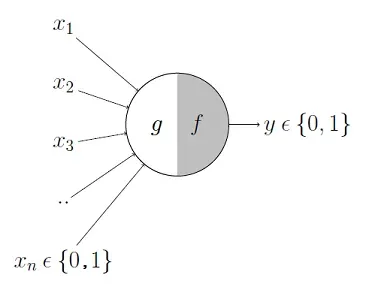
\includegraphics[width=0.5\textwidth]{Immagini/Generiche/ModelloNeurone.png}
%     \caption{Rappresentazione del modello}
%     \label{fig:modelloNeurone}
%     %Figura 2.1: Esempio schematico di un neurone
% \end{figure}
\begin{figure}[H]
    \centering
    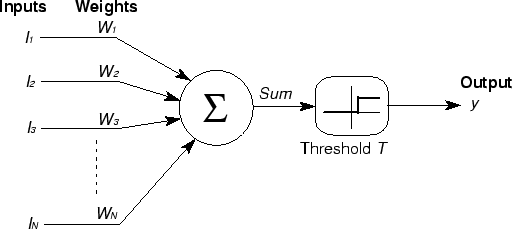
\includegraphics[width=0.75\textwidth]{Immagini/Generiche/PercettroneBinario.png}
    \caption{Rappresentazione del modello \cite{IMAMGINE_MODELLO_MAT_NEURONE_GENERALE_PERCETTONE}}
    \label{fig:modelloNeurone}
    %Figura 2.1: Esempio schematico di un neurone
\end{figure}

L’elaborazione prevedeva nel moltiplicare ogni input per un valore specifico, detto “peso”. 
I risultati di queste moltiplicazione venivano poi sommati. 
Se tale somma supera una certa soglia, allora il neurone attivava la 
propria uscita. Formalmente, questa operazione può essere descritto come
\cite{MODELLO_E_FUNZIONAMNETO_REURONE_BIOLOGICO}:

\begin{equation}
    g(x_1, x_2,\dots,x_n) = g(X) = \sum_{i=1}^{n}x_i \cdot w_i
\end{equation}
\begin{equation}
    y = f(g(X)) =
    \begin{cases} 
    1 & \text{se } g(X) \ge \theta, \\ 
    0 & \text{se } g(X) < \theta.
    \end{cases}
\end{equation}

\newpage
Dove:
\begin{itemize}
    \item $ \theta $ = soglia di attivazione
    \item $ y $ = output attivo/spento (1/0)
    \item $ x_i $ = i-esimo ingresso attivo/spento (1/0)
    \item $ w_i $ = i-esimo peso
\end{itemize}




% \begin{equation}
%     y =
%     \begin{cases} 
%     1 & \text{se } \sum_{i=1}^n w_i x_i \geq \theta, \\ 
%     0 & \text{altrimenti}.
%     \end{cases}
% \end{equation}


La distribuzione dei valori dei pesi varia in  base all’importanza 
dell’ingresso: un ingresso importante avrà un peso elevato, a 
differenza di uno meno importante che avrà un valore inferiore. 
Tuttavia, tale modello non si rivelò molto pratico, in quanto, per avere i valori 
desiderati, bisognava impostare manualmente pesi e connessioni.
Alcune semplici operazioni logiche che possono essere eseguite con questo modello sono 
\cite{STORIA_PERCETTONE}:

\begin{itemize}
    \item \textbf{AND$(x_1, x_2,\dots x_n)$}: il neurone si attiva 
    solo se tutti gli input sono attivi. Ovvero, se consideriamo 2 
    input, è necessario che $y \ge 2 $, poiché ogni input attivo da un 
    contributo di 1 e la somma è 2.

    \item \textbf{OR$(x_1, x_2,\dots x_n)$}: il neurone si attiva se 
    almeno uno degli input è attivo. Ovvero, considerando 2 input, è 
    necessario che $y \ge 1 $, poiché basta un neurone attivo che dia un 
    contributo di 1.
 
\end{itemize}

\section{Il Percettrone}
Solo successivamente nel 1958, Frank Rosenblatt, uno psicologo statunitense, propose il
modello \textbf{perceptron} (percettrone), in un report intitolato “The Perceptron: A Perceiving and Recognizing Automaton”.
Questo modello è considerato come una delle prime architetture di reti neurali artificiali 
che riprende la logica utilizzata nel modello di McCulloch e Pitts, ma leggermente più complesso.
L’innovazione principale rispetto al modello di McCulloch-Pitts riguardava l'utilizzo di valori numerici reali, 
come input, superando la limitazione all'impiego esclusivo di dati binari. 
Inoltre, i valori dei pesi associati a ciascun input venivano appresi mediante una 
regola di apprendimento che 
tiene conto della differenza tra output del neurone e output desiderato
\cite{ASPETTI_APPRENDIMENTO_PERCETTONE,STORIA_PERCETTONE,ARTICOLO_PERCETTONE,
IMAMGINE_MODELLO_MAT_NEURONE_GENERALE_PERCETTONE}.

\begin{figure}[H]
    \centering
    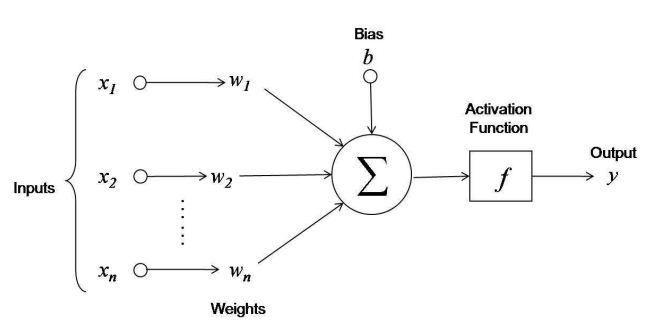
\includegraphics[width=0.75\textwidth]{Immagini/Generiche/neuron_representation_cornell.jpeg}
    \caption{Rappresentazione del modello \cite{IMMAGINE_PERCETTRONE_ASPETTI}}
    \label{fig:modelloNeurone2}
    %Figura 2.1: Esempio schematico di un neurone
\end{figure}

Un percettrone può essere visto come un classificatore lineare; cioè un algoritmo 
che classifica l'input separando due categorie tracciando una linea retta (o un iperpiano in spazi a dimensioni superiori).
Per questa ragione, il perceptron è considerato un passo cruciale nello sviluppo 
degli algoritmi di apprendimento automatico. 

Matematicamente, il funzionamento del perceptron può essere espresso attraverso 
le seguenti formule \cite{FORMULE_PERCETTRONE}:
\begin{equation}
    z = \sum_{i=1}^{n} w_i x_i + b = (x_1 \cdot w_1)\ + (x_2 \cdot w_2)\ + ...\ + (x_n \cdot w_n) + b 
\end{equation}
\begin{equation}
    y = \hat{y}= f\left(z\right)
\end{equation}

Dove:
\begin{itemize}
    \item \(x_i\) rappresenta il valore di ciascun input;
    \item \(w_i\) è il peso associato all'input \(x_i\);
    \item \(b\) è il bias, un termine aggiuntivo che permette di traslare la funzione di attivazione;
    \item \(f\) è una funzione di attivazione, generalmente una soglia (ad esempio, una funzione scalino) che 
    determina l'output finale del modello. Una delle funzioni più utilizzate è l'\textbf{Heaviside step function}:
    \[f(z) =
        \begin{cases} 
        1 & \text{if } z \ge 0, \\ 
        0 & \text{if } z < 0.
        \end{cases}
    \]
    
    \item \(y\) rappresenta l'output del modello, che spesso viene indicato anche come \(\hat{y}\) per denotare un valore stimato o predetto.
\end{itemize}

Spesso, per rappresentare le operazioni in una maniera più compatta e generalizzata, si adotta 
una rappresentazione vettoriale, in cui i valori degli input e dei pesi sono rappresentati come segue:
\[
    \mathbf{X} = \begin{bmatrix} x_1 \\ x_2 \\ \vdots \\ x_n \end{bmatrix}, \quad
    \mathbf{W} = \begin{bmatrix} w_1 \\ w_2 \\ \vdots \\ w_n \end{bmatrix}
\]
    
%i valori di input (\(x_i\)) sono rappresentati dal vettore \(\mathbf{X}\), mentre i pesi (\(w_i\)) sono rappresentati dal vettore \(\mathbf{W}\).
Utilizzando questa notazione, la formula che descrive il funzionamento del perceptron in 
forma vettoriale è definita come:

\begin{equation}
    \begin{split}
        \hat{y} &= f\left( \mathbf{X}^\top \mathbf{W} + b \right)
        = f\left( 
        \begin{bmatrix} x_1 & x_2 & \cdots & x_n \end{bmatrix} \cdot
        \begin{bmatrix} w_1 \\ w_2 \\ \vdots \\ w_n \end{bmatrix}
        + b
        \right)%= \\
        % &= f\left( (x_1 \cdot w_1) + (x_2 \cdot w_2) + \dots + (x_n \cdot w_n) + b \right) = f(z + b)
    \end{split}
    \label{eq:formulaPercettroneVettoriale}
\end{equation}

\subsection{L'Algoritmo di Apprendimento del Percettrone}
Rosenblatt dimostrò che l’algoritmo di apprendimento del percettrone converge se le
 due classi sono linearmente separabili, ovvero se esiste un iperpiano lineare che separi
 correttamente le due classi.
L'algoritmo di apprendimento del percettrone si basa su un approccio iterativo di 
ottimizzazione dei pesi. Durante l'addestramento, i pesi vengono aggiornati sulla 
base dell'errore tra l'uscita prevista e l'uscita reale. Tale processo di aggiornamento 
dei pesi può essere descritto tramite la seguente regola 
\cite{APPRENDIMENTO_PRECETTRONE,ASPETTI_APPRENDIMENTO_PERCETTONE,IMAMGINE_MODELLO_MAT_NEURONE_GENERALE_PERCETTONE}:

\begin{equation}
    w_i = w_i + \eta(y - \hat{y}) x_i
    \label{eq:apprendimentoPercettrone}
\end{equation}

dove:
\begin{itemize}
    \item \( \eta \) è una costante che determina il tasso di apprendimento. \\Questo 
    valore è noto anche come \textbf{learning rate};
    \item \( y \) è il valore atteso;
    \item \( \hat{y} \) è il valore predetto dal percettrone;
    \item \( x_i \) è l'input associato al peso \( w_i \).
\end{itemize}

\subsection{Implementazione di un percettrone}
Per comprendere il funzionamento di questo modello, proviamo a implementare un 
percettrone utilizzando un linguaggio di programmazione e 'addestrarlo' a distinguere 
i punti separati da una retta.

\hspace{0.25cm}

Per la parte di algebra lineare useremo la libreria \textbf{numpy}. Mentre per realizzare i
vari grafici useremo la libreria \textbf{matplotlib}.
\begin{lstlisting}
import numpy as np
import random
import matplotlib as plt
\end{lstlisting}

Basandosi sulle formule \eqref{eq:apprendimentoPercettrone} e \eqref{eq:formulaPercettroneVettoriale}, 
il percettrone può essere modelizzato nel seguente modo:

\begin{lstlisting}

    class Perceptron:

        def __init__(self, inputs: int) -> None:
            self.W: np.array = np.random.rand(inputs) 
            self.b: float = random.random()

        def heaviSideStep(self, z: float) -> int:
            return 1 if z >= 0.0 else 0

        def predict(self, X: np.array) -> int:
            z = np.dot(self.W, X) + self.b  # Somma pesata
            y_hat = self.heaviSideStep(z)
            return y_hat
        
        def train(self, lr: float, epochs: int, Y_train: np.array, X_train: np.array) -> Tuple[np.array, np.array]:
        
            train_losses: List[float] = []
            epoch_avg_loss: List[float] = []

            for epoch in range(epochs):
                epoch_loss: List[float] = []

                for i, X in enumerate(X_train):
                    y_hat = self.predict(X)

                    # Calcolo dell'errore
                    error = Y_train[i] - y_hat  

                    # Aggiornamento dei pesi e del bias
                    self.W += lr * error * X
                    self.b += lr * error

                    # Salva l'errore
                    epoch_loss.append(error)

                # Errore medio per epoca
                epoch_avg_loss.append(np.mean(epoch_loss))
                train_losses.extend(epoch_loss)

            return np.array(train_losses, dtype=np.float32), np.array(epoch_avg_loss, dtype=np.float32)
\end{lstlisting}

Per svolgere l'addestramento del percettrone, utilizziamo la funzione "train", alla 
quale forniamo un set di dati per il quale conosciamo già il risultato corretto. Durante 
l'addestramento, l'errore (o loss) viene calcolato per ogni esempio del set di 
dati, aggiornati di conseguenza i pesi ed il bias. 

I dati di esempio vengono utilizzati più volte. Ogni iterazione completa sul set di 
dati è chiamata \textbf{epoca} (epoch).

Durante questa procedura teniamo anche traccia di tutti i valori, in modo che poi possiamo 
utilizzarli per visualizzare l'andamento.
\newpage
Iniziamo a definire i parametri 
\begin{lstlisting}
N_TRAIN: int = 5000
N_TEST: int = 2000
INPUT_SIZE: int = 2
MIN: int = -2
MAX: int = 12

alpha: float = -2
x_offset: float = -5
y_offset: float = +5

X_TRAIN = np.random.uniform(MIN, MAX, (N_TRAIN, 2))  # N punti casuali (x, y)
X_TEST = np.random.uniform(MIN, MAX, (N_TEST, 2))
Y_TRAIN = np.array([1 if x2 > alpha*(x1 + x_offset) + y_offset else 0 for x1, x2 in X_TRAIN])


perceptron = Perceptron(inputs=INPUT_SIZE)
print("Pesi iniziali:", perceptron.W)
print("Bias iniziale:", perceptron.b)

\end{lstlisting}


% \begin{figure}[H]
%     \centering
%     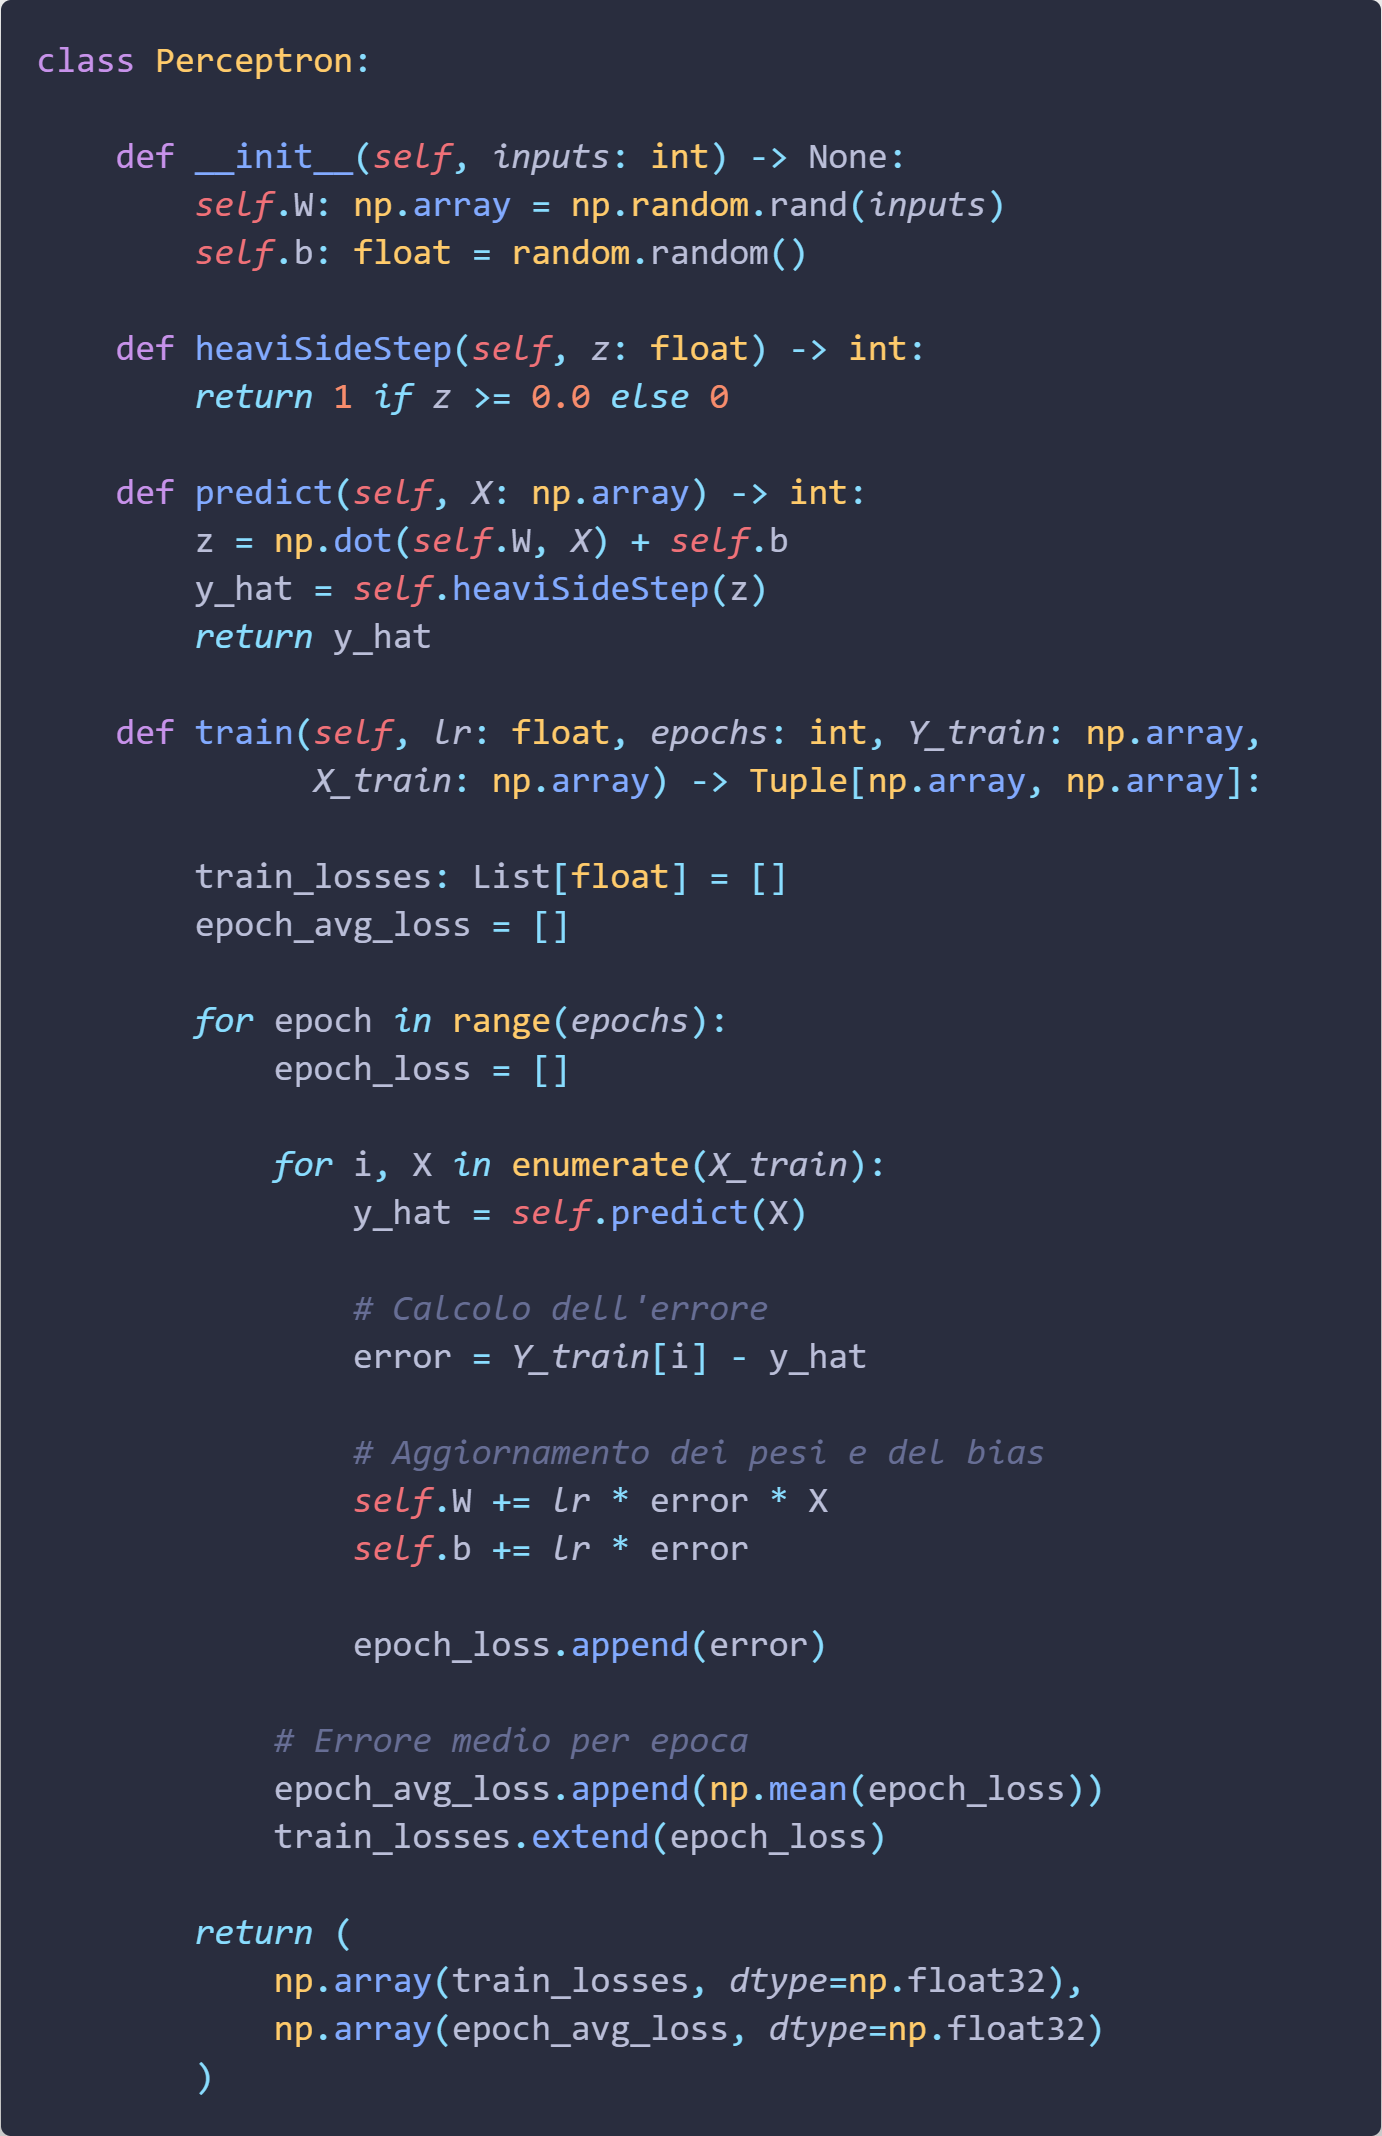
\includegraphics[width=0.8\textwidth]{Immagini/Codice/Perceptron.png}
%     %\caption{Grafico del problema dello XOR}
%     %\label{fig:Modellazione }
%     %Figura 2.1: Esempio schematico di un neurone
% \end{figure}

Pesi iniziali: [0.80801983, 0.46388153]
\newline
Bias iniziale: 0.7213280952626825

\hspace{0.25cm}

Ora chiamiamo la procedura per svolgere il training passandogli i vari parametri.
\begin{lstlisting}
# Training
train_losses, epoch_avg_loss = perceptron.train(lr=1e-3, epochs=30, Y_train=Y_TRAIN, X_train=X_TRAIN)

print("Pesi finali:", perceptron.W)
print("Bias finale:", perceptron.b)
\end{lstlisting}

Pesi finali: [0.06009108, 0.03008616]\\
Bias finale: -0.4496719047373185

\hspace{0.25cm}

Mentre per quanto riguarda il valore del piano tracciato dal percettrone, possiamo calcolarlo nel
seguente modo:
\begin{lstlisting}
slope = -perceptron.W[0] / perceptron.W[1]
intercept = -perceptron.b / perceptron.W[1]
\end{lstlisting}


\newpage

Così è come appare la classificazione dei casi di test prima della procedura di addestramento.

\begin{figure}[H]
    \centering
    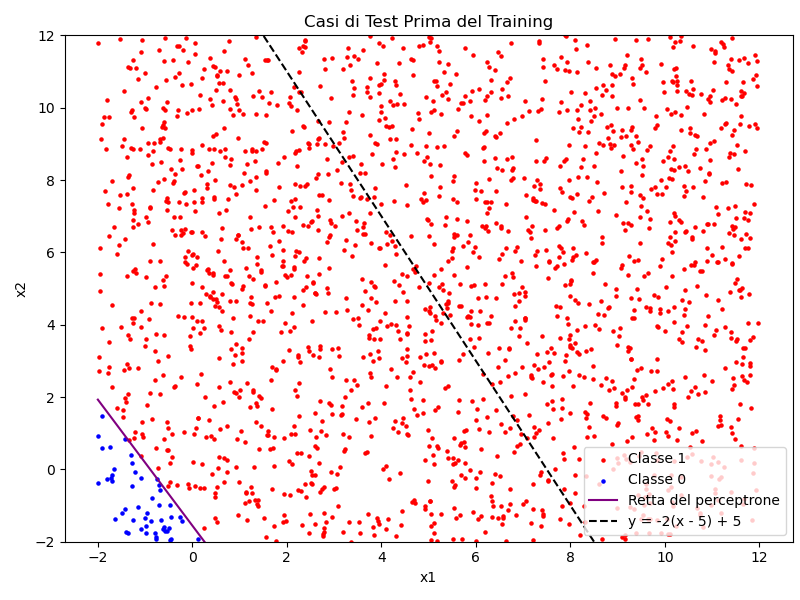
\includegraphics[width=0.80\textwidth]{Immagini/Grafici/EsempioApplicativoPercettrone_parte1.png}
    \caption{Grafico prima dell'addestramento}
    \label{fig:Modellazione1 }
    %Figura 2.1: Esempio schematico di un neurone
\end{figure}

La linea tratteggiata è la retta che voglio approssimare con il percettrone, mentre 
quella viola è la retta attuale del percettrone.
Finita la procedura di addestramento, il grafico appare così
\begin{figure}[H]
    \centering
    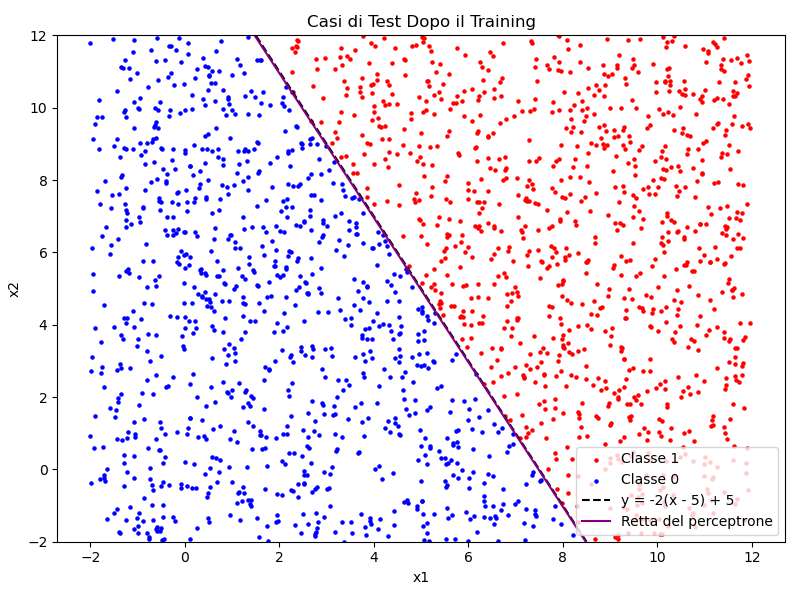
\includegraphics[width=0.80\textwidth]{Immagini/Grafici/EsempioApplicativoPercettrone_parte2.png}
    \caption{Grafico dopo l'addestramento}
    \label{fig:Modellazione2 }
    %Figura 2.1: Esempio schematico di un neurone
\end{figure}

Come si può osservare dei grafici \ref{fig:Modellazione1 } e \ref{fig:Modellazione2 }, 
il percettrone è riuscito ad "imparare" 
a classificare correttamente i punti di test, raggiungendo un precisione molto vicina al 100\%.

Il grafico sottostante mostra l'andamento dell'errore medio di ogni epoca 
durante la fase di addestramento.

\begin{figure}[H]
    \centering
    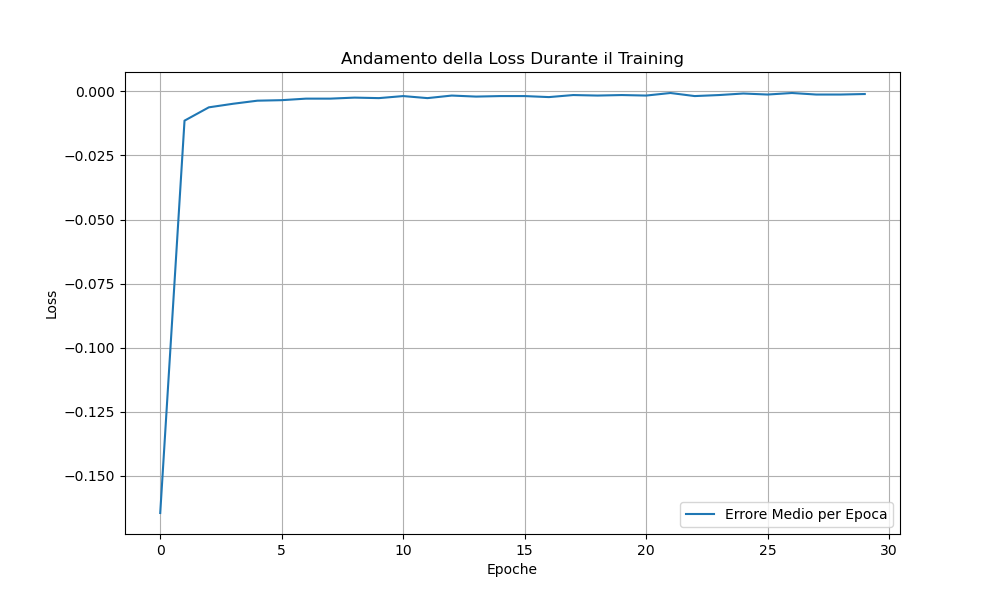
\includegraphics[width=1\textwidth]{Immagini/Grafici/EsempioApplicativoPercettroneLOSS.png}
    \caption{Grafico della loss}
    \label{fig:Modellazione3 }
    %Figura 2.1: Esempio schematico di un neurone
\end{figure}

% \begin{minted}[linenos, frame=lines, bgcolor=lightgray]{python}
% # Esempio di codice Python
% def somma(a, b):
%     """
%     Questa funzione restituisce la somma di due numeri.
%     """
%     return a + b

% print(somma(3, 5))
% \end{minted}





\subsection{Limiti del percettrone}
Nel 1969, Marvin Minsky e Symour A. Papert, nel loro libro “Perceptrons: an 
introducion to computational geometry”, dimostrarono matematicamente tutte le 
principali limitazioni 
del percettrone. 
Una di queste limitazioni riguardava l'incapacità del percettrone di gestire 
problemi non linearmente separabili \cite{ARTICOLO_LIMITI_PRECETTRONE}.
% , come dimostrato dal famoso esempio dell'operatore XOR, in quanto 
% quest'ultimo non è linearmente separabile.

La figura \ref{fig:XOR_GRAPH} mostra degli esempi di classificazione svolti dall'algoritmo del
percettrone per i problemi logici AND, OR e XOR. Graficamente, la retta di decisione
determinata dal percettrone riesce a classificare in maniera corretta ciascun elemento
in input nel caso dei problemi AND e OR. A differenza degli ultimi, è possibile notare
come una retta non sia sufficiente per separare le due classi nel problema XOR: ciò
è dovuto al fatto che tale rete riesce a classificare correttamente due classi 
linearmente separabili, ma non riesce a risolvere un problema di classificazione tra classi non
linearmente separabili, quale ad esempio il problema XOR.
L'unico modo consisterebbe nel dividere il piano in 3 aree utilizzando due rette di decisione, 
ma questo non è minimamente possibile utilizzando esclusivamente un solo percettrone 
\cite{LIMITI_PERCETTRONE, MODELLO_E_FUNZIONAMNETO_REURONE_BIOLOGICO}.

\begin{figure}[H]
    \centering
    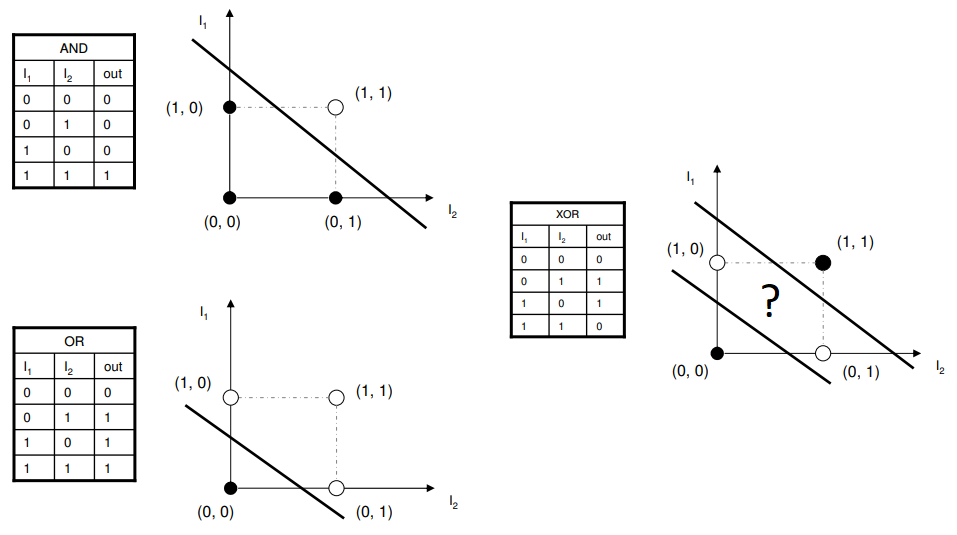
\includegraphics[width=1\textwidth]{Immagini/Grafici/graficiLimitiPercettrone.png}
    \caption{Esempi di classificazione \cite{LIMITI_PERCETTRONE}.}
    \label{fig:XOR_GRAPH}
    %Figura 2.1: Esempio schematico di un neurone
\end{figure}



% \begin{figure}[H]
%     \centering
%     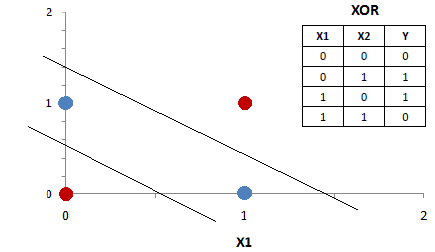
\includegraphics[width=0.60\textwidth]{Immagini/Grafici/Perceptron_XOR_v3.png}
%     \caption{Grafico del problema dello XOR}
%     \label{fig:XOR_GRAPH2}
%     %Figura 2.1: Esempio schematico di un neurone
% \end{figure}

Questa constatazione segnò l'inizio di un periodo noto come “Inverno delle IA”, durante 
il quale l'interesse per lo sviluppo delle reti neurali diminuì notevolmente.
Al fine di risolvere problemi più complessi, si cominciò ad interconnettere gli 
input dei neuroni artificiali con gli output di altri neuroni artificiali, creando 
una rete neurale a più livelli. Questo portò alla nascita 
del \textbf{Multi-layer Perceptron (MLP)} .


\section{Single-layer Perceptron (SLP)}
Il Single-layer Perceptro (percettrone a singolo layer)è un'estensione del 
percettrone singolo, in cui più percettroni sono in "pilati" per formare un unico strato (o layer). Questo permette all'SPL di poter
essere utilizzato per problemi di classificazione multiclasse.

I SLP furono utilizzati per diverse applicazioni durante gli anni '60, tuttavia, 
la scoperta dei limiti del perceptron (il libro di Minsky e Papert del 1969) 
fece calare rapidamente l'interesse per questi modelli, poiché non erano in 
grado di risolvere problemi non linearmente separabili \cite{ALL_SLP}.

\begin{figure}[H]
    \centering
    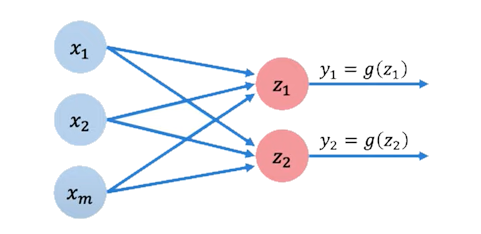
\includegraphics[width=0.60\textwidth]{Immagini/Generiche/SLP.png}
    \caption{Rappresentazione di un SLP}
    \label{fig:SingleLayerPerceptrons}
    %Figura 2.1: Esempio schematico di un neurone
\end{figure}
Come si può osservare, ogni nodo (percettrone) nello strato applica la stessa logica, 
ma in modo indipendente per calcolare diversi output.
\\Matematicamente, il funzionamento del Single-layer Perceptron è molto simile al funzionamento
del percettrone, infatti si ha che:
\begin{equation}
    z_i =  b_i + \sum_{j=1}^{m} w_{ij}\cdot x_j%= (x_1 \cdot w_1)\ + (x_2 \cdot w_2)\ + ...\ + (x_n \cdot w_n) + b 
\end{equation}
\begin{equation}
    \hat{y}_i= g\left(z_i\right)
\end{equation}

L'SLP può essere visto come una versione semplificata del MLP, pertanto non
ci soffermeremo ulteriormente.


